\documentclass[11pt,oneside]{book}

\usepackage[T1]{fontenc}
\usepackage[french]{babel}

\usepackage[utf8]{inputenc}
\usepackage{graphicx}
\usepackage{grffile}
\usepackage{longtable}
\usepackage{wrapfig}
\usepackage{rotating}
\usepackage[normalem]{ulem}
\usepackage{amsmath}
\usepackage{textcomp}
\usepackage{amssymb}
\usepackage{capt-of}
\usepackage[colorlinks=true,linkcolor=black,citecolor=black]{hyperref}
\usepackage{textgreek}
\usepackage{minted}
\usepackage{framed}
\usepackage{mdframed}
\usepackage{geometry}
\usepackage{titlesec}
\usepackage{pdfpages}
\usepackage{fancyhdr}
\usepackage{colortbl}
\usepackage{xcolor}
\usepackage[textwidth=16mm]{todonotes}

\newcommand{\as}[1]{\todo[color=green!40,size=\tiny,caption={}]{#1}}
\newcommand{\asi}[1]{\todo[inline,caption={},color=green!40]{#1}}

\newcommand{\hlink}[2]{\hyperlink{#1}{\color{magenta} #2}}

\geometry{
a4paper,
left=18mm,
right=18mm,
top=20mm,
bottom=20mm
}

\begin{document}


\includepdf[pages=-]{page1.pdf}

\pagestyle{empty}
\fontfamily{cmss}
\selectfont

\setlength{\parindent}{4mm}

\setcounter{tocdepth}{1}
\tableofcontents
\pagenumbering{gobble}

\chapter{Introduction}
\pagenumbering{arabic}
\setcounter{page}{1}
\pagestyle{fancy}
\fancyhf{}
\cfoot[\thepage]{\thepage}

Ce projet nous a été proposé par l’équipe \href{https://www-intuidoc.irisa.fr/}{IntuiDoc} de l’\href{https://www.irisa.fr/}{IRISA}, en étroite collaboration avec la startup \href{http://www.doptim.eu}{Doptim} et avec le soutien de Jean-Yves LE CLERC, conservateur du patrimoine aux \href{http://archives.ille-et-vilaine.fr/fr}{archives départementales} d'Ille-et-Vilaine. Tout au long de l’année, nous serons encadrés par Bertrand COÜASNON, enseignant-chercheur membre d'IntuiDoc, Erwan FOUCHÉ, chef de projet chez \href{https://www.soprasteria.com/fr}{Sopra Steria}, Julien BOUVET, ingénieur chez Sopra Steria également. Nous serons aussi accompagnés par Sophie TARDIVEL, responsable et \textit{data scientist} chez Doptim.

\paragraph{}
Dans ce rapport, nous rappellerons le contexte du projet qui justifie certains choix de conception. Nous décrirons ensuite l’architecture logicielle générale de notre projet ainsi que les diagrammes de séquences illustrant le fonctionnement interne de ce dernier. Puis, nous décrirons plus en détail les deux itérations prévues, la première répondant simplement au cahier des charges, la seconde complétant l'ensemble des fonctionnalités décrites dans le rapport de spécification, et donnant plus d'importance à l'ergonomie de la solution logicielle.

% ---

\chapter{Spécifications fonctionnelles}

\section{Spécifications générales}

\subsection{Aspect général du projet}

Le projet se découpe en quatre grandes parties qui sont :
\begin{itemize}
	\item la préparation des données ;
	\item le stockage des données dans une BDD ;
	\item l'interface avec le reconnaisseur ;
	\item l'IHM.
\end{itemize}

\paragraph{}
Ces parties sont résumées sur le schéma 1, déjà abordé dans le rapport de
pré-étude.

\paragraph{}
\begin{mdframed}[frametitle={Figure 1 : Décomposition du projet (mode apprentissage)}, innerbottommargin=10]
\begin{center}
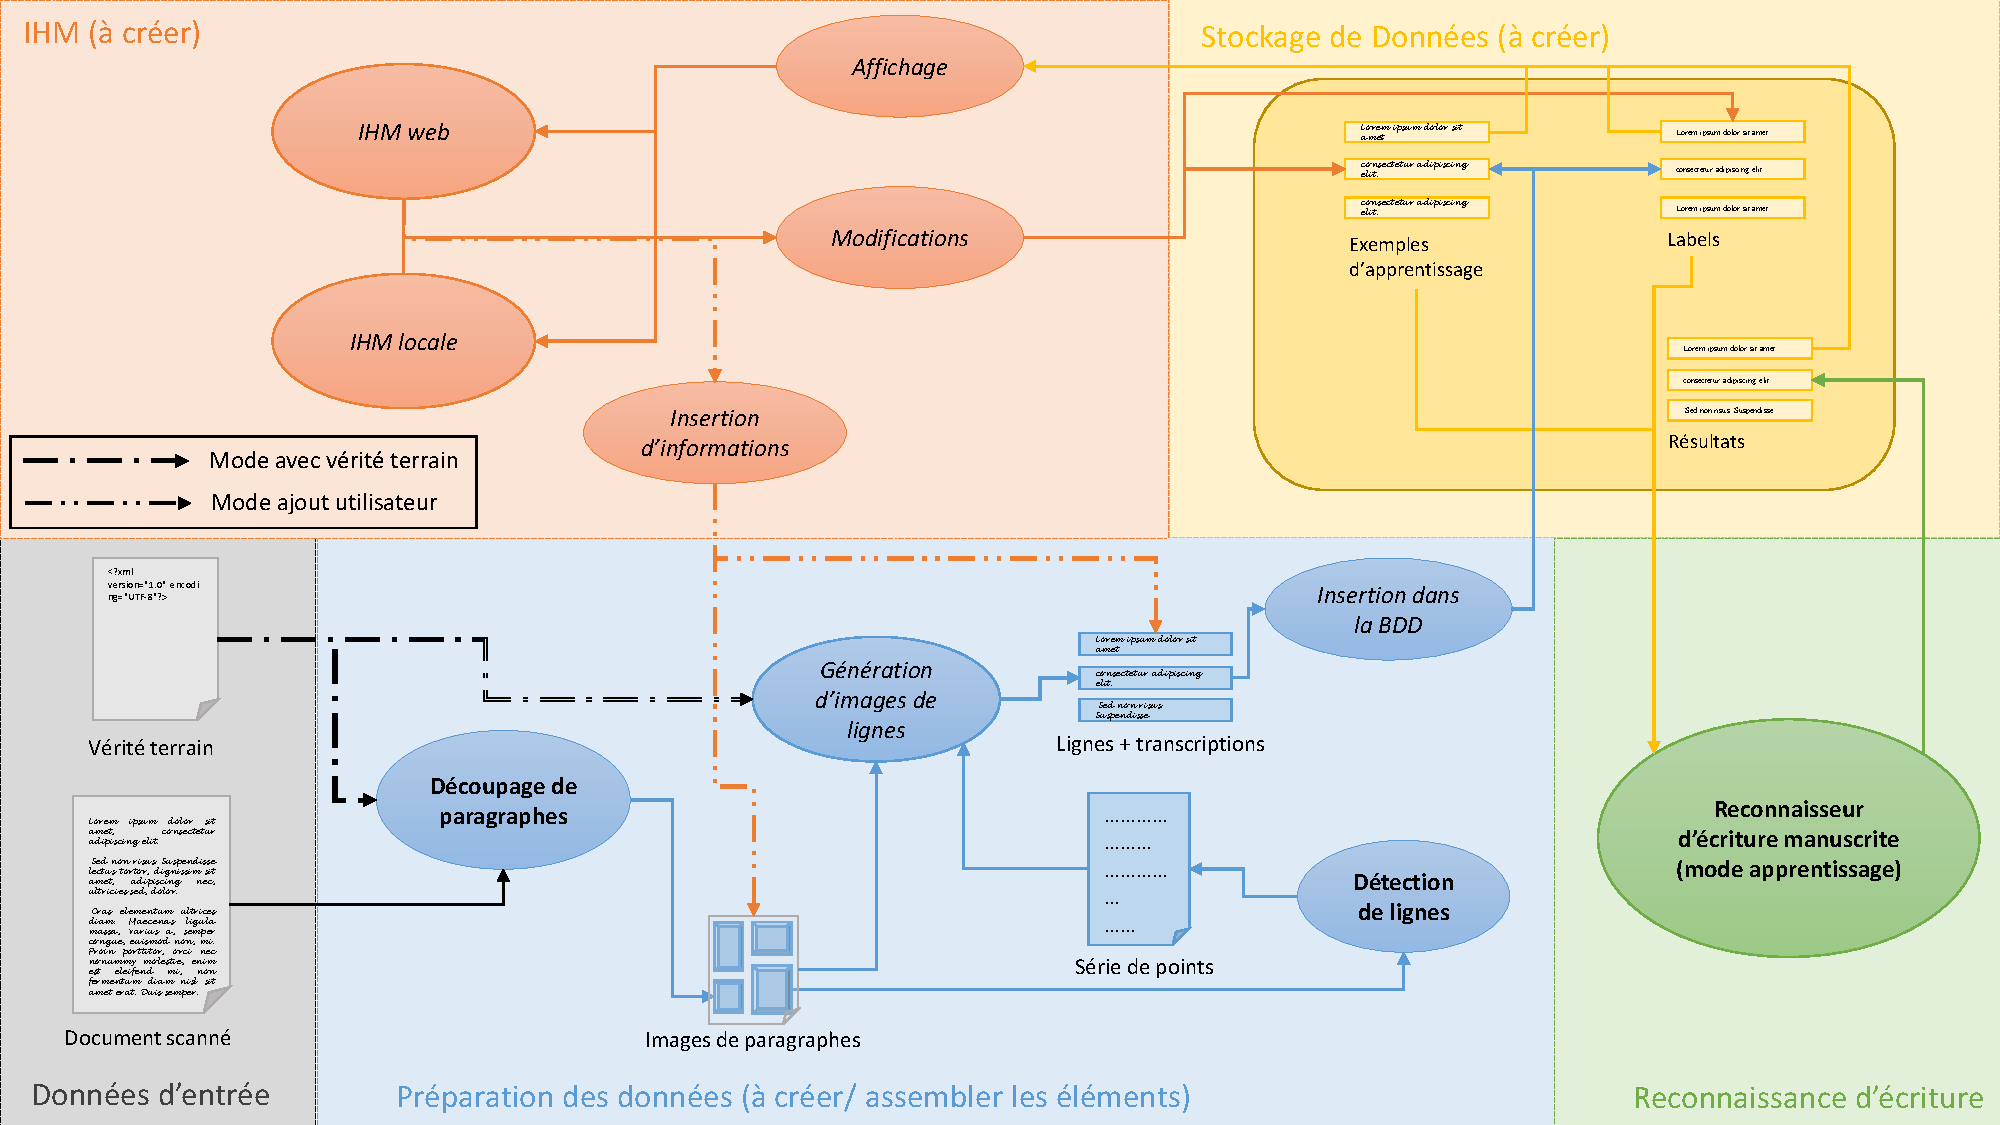
\includegraphics[width=\linewidth]{schema_mode1.1.pdf}
\end{center}
\end{mdframed}

\paragraph{}
Le projet se présente sous la forme d’un programme, principalement écrit en
\href{http://scala-lang.org}{Scala}. En effet, lors du précédent rapport,
nous avions déjà évoqué ce choix personnel, qui permet de travailler à la
fois avec un langage fonctionnel et avec la JVM. Par la suite tous les éléments
décrits seront donc considérés comme écrits en Scala, et pour toute exception,
le langage utilisé sera précisé.

\paragraph{}

La partie découpe de documents prend en entrée des documents scannés contenant
de l’écriture manuscrite, en extrait les informations contenues sous la forme
de couples imagette-transcription et les stocke dans la BDD. Le
\textit{framework} de gestion de bases de données utilisé est codé en Java.
Les langages Scala et Java étant interopérables, car tournant tous deux sur la
JVM, notre code Scala est donc compatible avec ce \textit{framework}. Le code
de notre logiciel concernant la base de données sera écrit en Java.

\paragraph{}
Ces informations stockées sont mises à disposition d’un classifieur, pour qu’il
puisse s'entraîner sur celles-ci. Ce classifieur ne fait pas partie du cadre de
l’application, mais vient se greffer à celle-ci. Le programme doit donc faire
en sorte que les données de la BDD puissent être accessibles par le classifieur.
Le classifieur n’étant pas intégré au programme, il peut être changé à tout
moment. L’application doit néanmoins pouvoir le faire fonctionner selon 3 modes :
apprentissage, évaluation et production. Les données stockées dans la base sont
ainsi divisées en sous-ensembles, chacun correspondant à un mode de
fonctionnement.

\paragraph{}
Le tout est géré par l’utilisateur grâce à une interface Web, en JavaScript
pour une plus grande accessibilité et une meilleure portabilité. Ce choix a
également pour but de faciliter l’évolution de l’application vers une solution
multi-utilisateurs distants, où plusieurs personnes s‘y connecteraient via
Internet. Chaque partie sera expliquée plus en détails dans la suite du rapport.

\subsection{Côté utilisateur}

Le logiciel à créer fonctionnera donc suivant plusieurs modes de fonctionnement :
\begin{itemize}
	\item apprentissage ;
	\item évaluation ;
	\item production.
\end{itemize}

\paragraph{}
Les trois modes ne sont pas à implémenter avec la même priorité, seul le mode
apprentissage est nécessaire pour obtenir un résultat fonctionnel. Les deux
modes suivants sont à implémenter suivant le temps restant.

\paragraph{}
Le mode apprentissage a pour objectif de faire apprendre un système de
reconnaissance d’écriture. Le logiciel génère une base d’apprentissage pour un
système de reconnaissance d’écriture manuscrite et fournit les données
produites en entrée du reconnaisseur. Celui-ci peut alors les utiliser pour
apprendre à retranscrire correctement du texte.

\paragraph{}
Du point de vue de l'utilisateur du logiciel, par l’intermédiaire de l’IHM, il
peut :
\begin{enumerate}
\item charger un document dans la base de données, accompagné d’une vérité
terrain ;
\item charger un document dans la base sans vérité terrain ;
\item annoter ledit document pour lui associer une nouvelle transcription ;
\item lancer l’apprentissage du système de reconnaissance ;
\item modifier les données contenues dans la base :
\begin{enumerate}
\item supprimer un document ;
\item déplacer un document vers un autre sous-ensemble ;
\end{enumerate}
\item changer de mode de fonctionnement.
\end{enumerate}

\newpage

\begin{mdframed}[frametitle={Figure 2 : Diagramme de cas d'utilisation (mode apprentissage)}, innerbottommargin=10]
\begin{center}
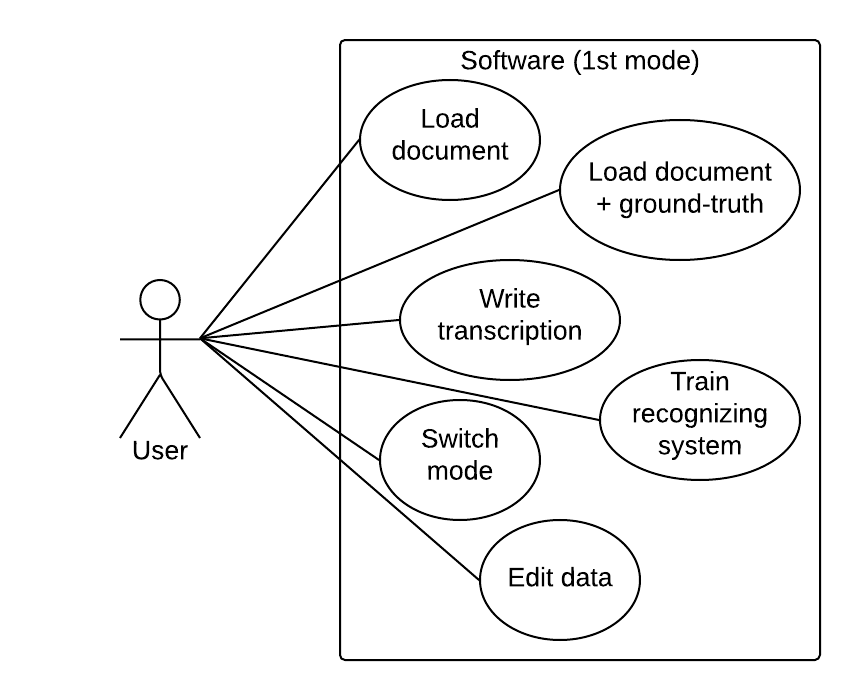
\includegraphics[scale=0.6]{Usecase_1.png}
\end{center}
\end{mdframed}

\paragraph{}

Le mode évaluation a pour objectif d’évaluer un système de reconnaissance. Ce
mode est en général utilisé après avoir effectué un apprentissage avec le
reconnaisseur. Il permet de vérifier l’efficacité de l’apprentissage effectué.

\paragraph{}

Dans ce mode, toujours par l’intermédiaire de l’IHM, l’utilisateur peut :
\begin{enumerate}
\item charger un document, accompagné d’une vérité terrain (la vérité terrain
est obligatoire dans ce mode de fonctionnement, pour que l’évaluation soit
correcte) ;
\item lancer l’évaluation du système de reconnaissance ;
\item modifier les données contenues dans la base :
\begin{enumerate}
\item supprimer un document ;
\item déplacer un document vers un autre sous-ensemble ;
\end{enumerate}
\item changer de mode de fonctionnement.
\end{enumerate}

\paragraph{}

\begin{mdframed}[frametitle={Figure 3 : Diagramme de cas d'utilisation (mode évaluation)}, innerbottommargin=10]
\begin{center}
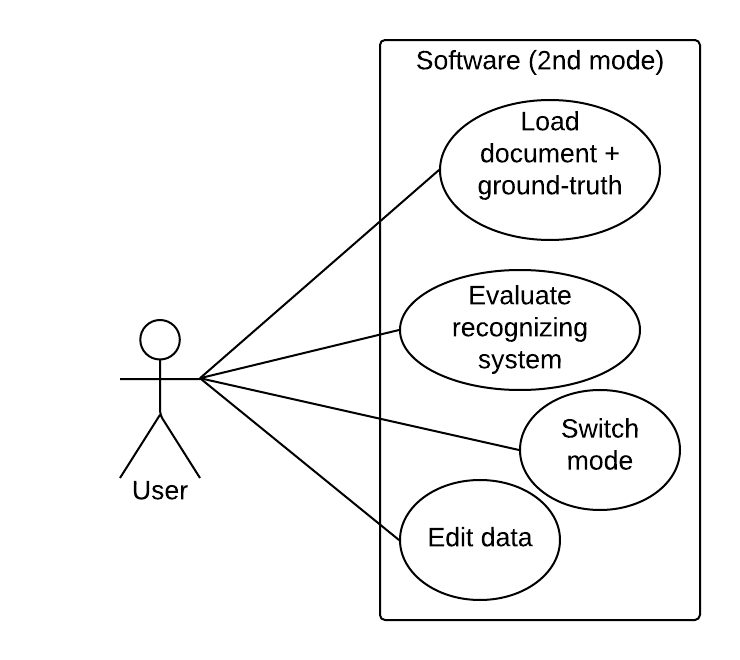
\includegraphics[scale=0.6]{Usecase_2.png}
\end{center}
\end{mdframed}

\paragraph{}
Le mode production a pour objectif d’utiliser un système de reconnaissance afin
d’obtenir une transcription pour des documents n’en ayant pas. Ce mode est en
général utilisé sur un reconnaisseur entraîné, dont l’apprentissage a été
évalué, et ayant donc obtenu de bons résultats. Il s’agit également d’un mode
de démonstration, permettant d’utiliser le reconnaisseur de manière ludique.
Il pourra être utilisé lors de la démonstration de fin de projet.

\paragraph{}
Dans ce mode, via l'intermédiaire de l’IHM, l’utilisateur peut :
\begin{enumerate}
\item charger un document sans vérité terrain ;
\item écrire une transcription manuellement, pour compléter ou corriger la
transcription du reconnaisseur ;
\item jouer à des mini-jeux en utilisant le reconnaisseur (le contenu des
mini-jeux n’a pas encore été établi, cette option étant annexe au projet) ;
\item modifier les données contenues dans la base :
\begin{enumerate}
\item supprimer un document ;
\item déplacer un document vers un autre sous-ensemble ;
\end{enumerate}
\item changer de mode de fonctionnement.
\end{enumerate}

\paragraph{}
\begin{mdframed}[frametitle={Figure 4 : Diagramme de cas d'utilisation (mode production)}, innerbottommargin=10]
\begin{center}
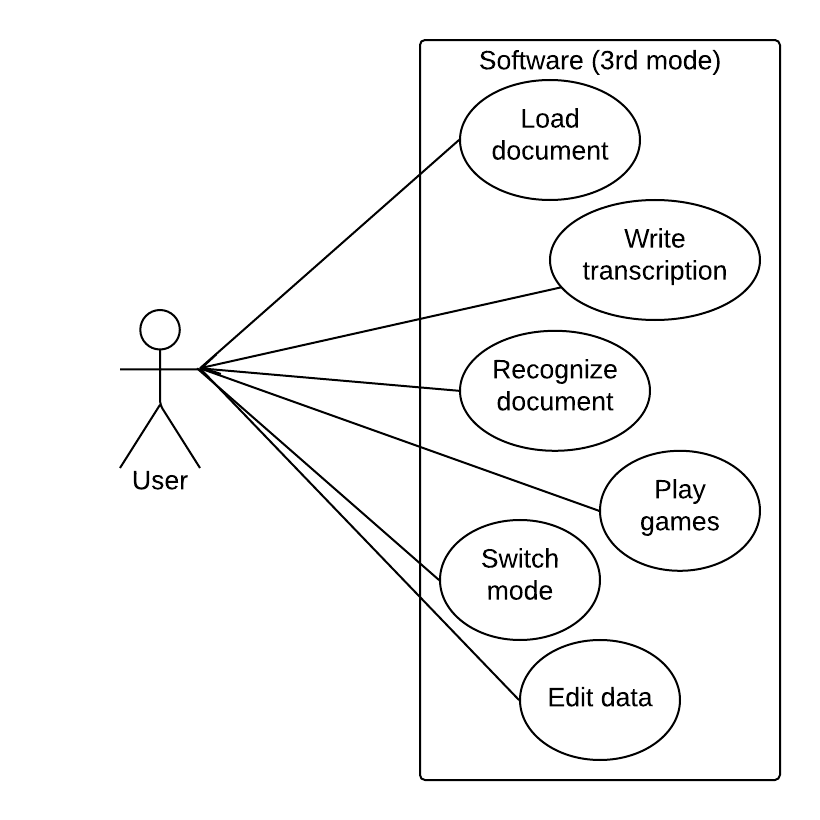
\includegraphics[scale=0.6]{Usecase_3.png}
\end{center}
\end{mdframed}

\paragraph{}
Le logiciel ne possède pas de système de reconnaissance d’écriture intégré.
Cette partie, comme précisé précédemment, y est simplement greffée. Il n’est
pas prévu de pouvoir changer de reconnaisseur via l’interface graphique, cette
opération étant rare et pouvant même ne jamais avoir lieu au cours de la vie du
logiciel. Néanmoins, il doit être possible pour un développeur de système de
reconnaissance d’écriture manuscrite utilisant notre logiciel de changer le
reconnaisseur. Cette possibilité sera donc incluse dans le projet.

\paragraph{}
\begin{mdframed}[frametitle={Figure 5 : Diagramme de cas d'utilisation (pour développeur)}, innerbottommargin=10]
\begin{center}
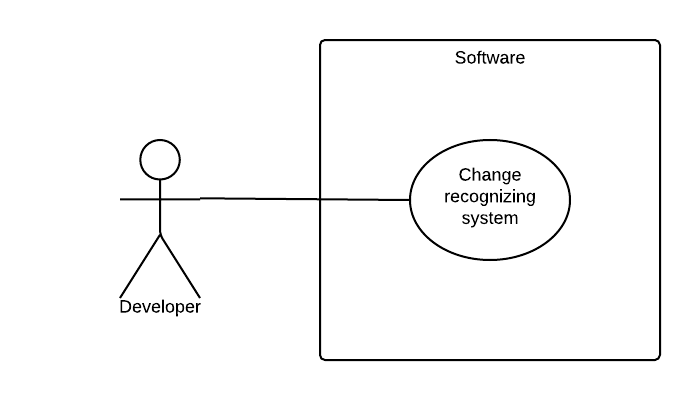
\includegraphics[scale=0.7]{Usecase_Dev.png}
\end{center}
\end{mdframed}

    
\section{Préparation des données}

Cette partie du projet a pour but de réaliser un premier traitement sur les
données d’entrée. Ces données sont aux formats GEDI et PiFF, présentés dans
le dernier rapport (une courte définition est rappelée en annexe 1). 
Nous devons fournir un logiciel qui soit capable de
traiter ces formats (\textbf{PR\_FO\_1} et \textbf{PR\_FO\_2}). Nous avons validé
la proposition que nous avions faite, qui était de choisir PiFF comme format
de traitement unique. Nous fournirons donc un convertisseur de GEDI vers PiFF,
et nous garantirons par modélisation logicielle la possibilité pour les futurs
utilisateurs d’écrire d’autres convertisseurs des formats de leur choix vers
PiFF s’ils le souhaitent (\textbf{GEN\_EVOL}).

\paragraph{}
En exploitant le fichier PiFF, ce module du projet génèrera les imagettes qui
formeront les exemples. Les coordonnées utilisées pour la découpe d’image seront
calculées grâce au polygone identifiant le paragraphe présent dans le fichier
d’entrée, ainsi que les détecteur de lignes. Cette découpe pourra être réalisée
soit en lignes, soit en paragraphes, ce qui correspond à deux reconnaisseurs
différents à utiliser par la suite. Les deux options seront
disponibles sur le logiciel.

\paragraph{}
Nous devrons récupérer la vérité terrain si elle existe dans le fichier d’entrée,
afin de pouvoir l’afficher sur l’IHM et permettre à l’utilisateur de la corriger
ainsi qu’au reconnaisseur de s’entraîner avec, en lui fournissant des exemples
que notre logiciel aura créés en associant les imagettes à leur transcription.

\section{Stockage des données}

\subsection{Objectifs du système de stockage}

Le principal objectif du système de stockage est de pouvoir stocker les données
traitées par notre logiciel. Ainsi, il doit être possible de pouvoir stocker
des imagettes associées à leur transcription (vérité terrain) (\textbf{STO\_VER}).
On doit aussi pouvoir stocker des imagettes associées à une transcription établie
par l’utilisateur (\textbf{STO\_USR}). On devra également pouvoir stocker les
données obtenues par le système de reconnaissance d’écriture manuscrite qui aura
été entraîné grâce à la base d’apprentissage que notre logiciel lui aura fourni.
Ainsi, il faudra aussi stocker des imagettes associées à leur transcription
générée par le reconnaisseur (\textbf{STO\_REC}).

\paragraph{}
En plus de stocker les données, la partie base de données devra pouvoir
communiquer facilement avec les autres blocs de notre logiciel (IHM et
préparateur de données). Il faudra ainsi fournir une bibliothèque afin 
de pouvoir accéder aux données (\textbf{STO\_SEL}) de la base, les modifier
(\textbf{STO\_UPD}), en ajouter (\textbf{STO\_INS}) ou en supprimer
(\textbf{STO\_DEL}).

\section{Interface avec le reconnaisseur}

Cette partie du projet a pour but de faire le lien avec le système de
reconnaissance d’écriture. Située entre la BDD et le reconnaisseur,
l’interface permet de faire transiter des informations entre les deux, sans
contraintes de format. Elle convertit les données stockées en données
intelligibles pour le reconnaisseur (\textbf{IR\_CV}).

\paragraph{}
Pour tester notre programme, nous avons un reconnaisseur d’écriture
manuscrite nommé
\href{https://github.com/jpuigcerver/Laia/tree/master/egs/iam}{Laia} à notre
disposition. Ce reconnaisseur prend en format d’entrée des fichiers dans un
format spécifique. Dans le cadre d'un approfondissement du projet, nous
pourrons concevoir un programme qui transforme les
données stockées dans notre base au format adéquat pour que Laia puisse
apprendre. Notre programme ayant pour vocation à être utilisé par différents
systèmes de reconnaissance, nous allons laisser le code de ce programme
\textit{open source} pour que n’importe qui puisse définir son propre
formateur de données (\textbf{IR\_OS}).

\paragraph{}
Notre logiciel pourra également, via cette interface, lancer
l’apprentissage du système de reconnaissance (\textbf{IR\_AP}), lancer une
évaluation (\textbf{IR\_EV}) et lancer une transcription de document
(\textbf{IR\_TR}).


\section{Interface Homme-Machine}

\subsection{Page d'édition des annotation}

La page d’édition des annotations présente trois modes d’édition différents :
un mode sans vérité terrain disponible au départ, un mode de correction des
transcriptions de l’IA, et un mode de validation finale.

\subsubsection{Informations générales}

L’interface doit tout d’abord permettre de naviguer entre les différents
documents d’un même classeur pour permettre à l’utilisateur d’ouvrir un autre
manuscrit (\textbf{PEA\_GEN\_1}). Elle doit également permettre de naviguer
entre les différentes pages du manuscrit en cours d’annotation
(\textbf{PEA\_GEN\_2}).

\paragraph{}
L’interface possède trois modes d’édition des annotations différents et doit
donc permettre de naviguer entre les modes de façon ergonomique et claire
(\textbf{PEA\_GEN\_3}).

\paragraph{}
Afin de basculer vers la page d’édition des zones de découpe, elle doit
posséder un bouton intitulé “modifier les zones du manuscrit”
(\textbf{PEA\_GEN\_4}). Pour plus de clarté, l’interface doit posséder une zone
montrant la page découpée afin de localiser les zones de découpe du manuscrit,
avec la zone en cours d’annotation figurant en une couleur différente
(\textbf{PEA\_GEN\_5}).

\paragraph{}
La zone principale de l’interface doit afficher la liste des imagettes du
manuscrit découpé (\textbf{PEA\_GEN\_6}). Chaque imagette est suivie de
l’annotation correspondante. Le couple imagette-transcription est chargé
depuis la base de données. Lorsque la vérité-terrain d’une imagette est
modifiée, les modifications sont aussitôt envoyées à la base de données
(\textbf{PEA\_GEN\_7}). En outre, si une imagette ou sa transcription n’est
pas pertinente pour l’ensemble d’apprentissage, le couple
imagette-transcription peut être supprimé de la base de données à l’aide d’un
bouton prévu à cet effet (\textbf{PEA\_GEN\_8}).

\paragraph{}
L’utilisateur peut également ajouter à la base de données des documents avec
ou sans transcription (\textbf{PEA\_GEN\_9}) et exporter les données validées
afin de lancer un nouvel apprentissage (\textbf{PEA\_GEN\_10}).

\subsubsection{Mode annotations}

Dans ce mode, aucune vérité terrain n’est disponible. L’utilisateur doit donc
annoter à la main tout le manuscrit afin de générer l’ensemble
d’apprentissage. Pour faciliter le travail de l’utilisateur, à l’ouverture de
la page, le curseur est placé sur la première imagette ne possédant pas de
transcription (\textbf{PEA\_MA\_1}). Puis, pendant l’édition des vérités
terrain, un simple appui sur la touche \textbf{Entrée} permet de positionner le
curseur sur l’annotation suivante afin de faciliter la navigation et de réduire
le temps passé à l’édition des transcriptions (\textbf{PEA\_MA\_2}). Enfin,
l’interface doit proposer un bouton permettant de basculer vers la prochaine
imagette sans vérité-terrain (\textbf{PEA\_MA\_3}). Cela est utile dans le cas
où les transcriptions manquantes sont éparpillées et ne se suivent pas.

\subsubsection{Mode correction de la reconnaissance}

Dans ce mode, l’utilisateur doit corriger les annotations proposées par l’IA
à la suite de son apprentissage. En partant du principe que les transcriptions
proposées par l’IA sont relativement fiables et pour diminuer le temps passé
à la validation, un simple appui sur \textbf{Entrée} valide les transcriptions
zone par zone et passe à la zone suivante (\textbf{PEA\_MCR\_1}). Si une
transcription est fausse, l’utilisateur doit pouvoir la modifier en cliquant
dessus pour y positionner son curseur et en effectuant ses modifications
manuellement (\textbf{PEA\_MCR\_2}).

\subsubsection{Mode validation}

Dans ce mode, la vérité terrain a été validée auparavant par l’utilisateur.
Il fait donc office de validation finale. L’interface propose une lecture
rapide pour ajouter des corrections si besoin. Ainsi, un simple appui sur
\textbf{Entrée} valide les transcriptions zone par zone (\textbf{PEA\_MV\_1}).
Si une transcription s’avère fausse, l’utilisateur doit pouvoir la modifier
en cliquant dessus et en effectuant ses modifications manuellement
(\textbf{PEA\_MV\_2}).

\subsection{Page de découpe des zones}

Cette page permet à l’utilisateur de définir et de modifier les différentes
zones qui découpent le manuscrit.

\subsubsection{Outils de découpe}

La page d’édition des zones offre plusieurs outils de découpe, d’édition des
zones et de navigation dans le manuscrit.
\begin{itemize}
\item l’outil “nouvelle sélection” crée une nouvelle zone à l’aide d’un
rectangle (\textbf{PDEC\_OD\_1}). Les rectangles qui définissent initialement
les zones doivent avoir des sommets dont on peut modifier la position pour
une découpe plus fine. Les zones ne sont donc pas limitées à des rectangles,
mais peuvent prendre la forme d’autres polygones (\textbf{PDEC\_OD\_2}) ;
\item l’outil “déplacer” déplace la zone sélectionnée sur le manuscrit
(\textbf{PDEC\_OD\_3}). Cela est utile quand l’utilisateur s’aperçoit que
plusieurs de ses zones sont mal positionnées. Il peut donc déplacer chaque
zone en un clic à l’aide de cet outil ;
\item l’outil “zoom +” permet de zoomer sur le manuscrit et “zoom -” de
dézoomer, afin de faciliter l’édition des zones (\textbf{PDEC\_OD\_4}) ;
\item l’outil “annuler” permet d’annuler la dernière action
(\textbf{PDEC\_OD\_5}) et l’outil “refaire” permet de refaire l’action
annulée précédemment (\textbf{PDEC\_OD\_6}) ;
\item l’outil “réinitialiser” supprime toutes les zones de la page pour
retourner au manuscrit vierge (\textbf{PDEC\_OD\_7}) en cas de travail erroné ;
\item afin de permettre à l’utilisateur de vérifier son travail au fur et à
mesure, l’interface de découpe doit proposer un outil “appliquer la détection
de lignes sur la zone” (\textbf{PDEC\_OD\_8}). Cet outil applique le détecteur
de lignes sur la zone sélectionnée, afin de voir quelles lignes sont détectées
pour vérifier que la zone est bien définie ;
\item enfin, l’outil “valider” valide la découpe et bascule vers la page
d’édition des annotations (\textbf{PDEC\_OD\_9}).
\end{itemize}

\subsubsection{Visualisation du manuscrit}

L’interface doit posséder un bouton de retour au menu principal
(\textbf{PDEC\_VM\_1}) ainsi qu’une zone de navigation dans les autres
documents pour permettre à l’utilisateur d’ouvrir un autre manuscrit
(\textbf{PDEC\_VM\_2}). Elle doit également permettre de naviguer entre les
différentes pages du manuscrit (\textbf{PDEC\_VM\_3}). Enfin, la zone de
visualisation doit pouvoir permettre à l’utilisateur de se déplacer sur le
manuscrit horizontalement et verticalement à l’aide d’un bouton de
défilement (\textbf{PDEC\_VM\_4}).


% ---

\chapter{Architecture logicielle}

\section{Description des modules}

\section{Interactions}

% ---

\chapter{Organisation du travail}

\section{Répartition des tâches}

Comme le projet peut être découpé en plusieurs blocs qui peuvent être
développés de manière presque indépendante, nous nous sommes répartis
par équipe sur chaque bloc. Certains blocs nécessitent
cependant une base provenant d’autres blocs pour faire des tests.
Par exemple, la partie IHM aura besoin d’une base de données pour
vérifier que la recherche d’imagettes dans celle-ci se déroule bien.
Nous allons donc commencer par développer des prototypes simplifiés
pour que tout le monde puisse améliorer sa partie. De plus, certains 
blocs ne représentent pas la même quantité de travail, certaines 
personnes sont donc réparties sur plusieurs blocs.

\paragraph{}
Voici la répartition que nous avons effectuée sur les différents blocs :

\begin{center}

\begin{tabular}{ | l | l | }
	\hline
	\multicolumn{2}{ | c | }{ \textbf{Bloc 1 : Préparation des données} } \\
	\hline
	\textbf{Spécification} & \textbf{Description} \\
	\hline
	PR\_FO\_1 & Traiter le format PiFF en interne dans le logiciel \\
	\hline
	PR\_FO\_2 & Fournir un convertisseur du format GEDI vers PiFF \\
	\hline
	PR\_TR\_1 & Intégrer une fonction de détection de lignes au logiciel \\
	\hline
	PR\_TR\_2 & Permettre un découpage des images en lignes \\
	\hline
	PR\_TR\_3 & Localiser les paragraphes \\
	\hline
	PR\_TR\_4 & Permettre un découpage des images en paragraphes \\
	\hline
	PR\_RE\_1 & Associer les images à leur transcription \\
	\hline
	PR\_RE\_2 & Associer la vérité terrain à une transcription \\
	\hline
	PR\_RE\_3 & Permettre de générer une vérité terrain si besoin, grâce à un reconnaisseur \\
	\hline
\end{tabular}

\paragraph{}
\begin{tabular}{ | l | l | }
	\hline
	\multicolumn{2}{ | c | }{ \textbf{Bloc 2 : Stockage des données} } \\
	\hline
	\textbf{Spécification} & \textbf{Description} \\
	\hline
	STO\_VER & Stocker des imagettes associées à une vérité terrain \\
	\hline
	STO\_USR & Stocker des imagettes associées à une transcription générée par l’utilisateur \\
	\hline
	STO\_REC & Stocker des imagettes associées à une transcription générée par un reconnaisseur  \\
	\hline
	STO\_SEL & Fournir des méthodes pour accéder aux données stockées  \\
	\hline
	STO\_UPD & Fournir des méthodes pour modifier les données stockées \\
	\hline
	STO\_INS & Fournir des méthodes pour pouvoir insérer des données à stocker \\
	\hline
	STO\_DEL & Fournir des méthodes pour pouvoir supprimer des données stockées \\
	\hline
\end{tabular}

\paragraph{}
\begin{tabular}{ | l | l | }
	\hline
	\multicolumn{2}{ | c | }{ \textbf{Bloc 3 : Interface avec le reconnaisseur} } \\
	\hline
	\textbf{Spécification} & \textbf{Description} \\
	\hline
	IR\_CV & Convertir les données au format d’entrée du reconnaisseur \\
	\hline
	IR\_AP & Fournir les données au reconnaisseur \\
	\hline
	IR\_EV & Pouvoir lancer une évaluation du reconnaisseur  \\
	\hline
	IR\_TR & Pouvoir lancer une transcription d’un document par le reconnaisseur   \\
	\hline
\end{tabular}

\newpage

\begin{tabular}{ | l | p{0.8\linewidth} | }
	\hline
	\multicolumn{2}{ | c | }{ \textbf{Bloc 4 : Interface avec l’utilisateur} } \\
	\hline
	\textbf{Spécification} & \textbf{Description} \\
	\hline
	PEA\_GEN\_1 & Valider un ensemble d'annotations \\
	\hline
	PEA\_GEN\_2 & Éditer manuellement les transcriptions \\
	\hline
	PEA\_GEN\_3 & Corriger les annotations proposées par un reconnaisseur externe à l'application \\
	\hline
	PEA\_GEN\_4 & Envoyer les modifications à la base de données lorsque la vérité-terrain d’une imagette est modifiée \\
	\hline
	PEA\_GEN\_5 & Ignorer un couple imagette-transcription s’il n’est pas pertinent \\
	\hline
	PEA\_GEN\_6 & Regrouper les documents en projets \\
	\hline
	PEA\_GEN\_7 & Sélectionner d’abord le projet puis le document sur lequel l’utilisateur veut travailler à l’ouverture de l’application \\
	\hline
	PEA\_GEN\_8 & Créer un nouveau projet \\
	\hline
	PEA\_GEN\_9 & Basculer vers la page de découpe des zones \\
	\hline
	PEA\_GEN\_10 & Basculer vers la page d’édition des annotations \\
	\hline
	PEA\_GEN\_11 & Basculer vers la page de validation des transcriptions \\
	\hline
	PDEC\_OD\_1 & Créer une nouvelle zone à l’aide d’un rectangle (outil "nouvelle sélection") \\
	\hline
	PDEC\_OD\_2 & Pouvoir modifier la position des sommets des rectangles \\
	\hline
	PDEC\_OD\_3 & Rajouter des sommets à la zone \\
	\hline
	PDEC\_OD\_4 & Changer le type de la zone avec un menu déroulant \\
	\hline
	PDEC\_OD\_5 & Déplace la zone sélectionnée sur le document (outil “déplacer”) \\
	\hline
	PDEC\_OD\_6 & Zoomer et dézoomer sur le document (outils “zoom +” et “zoom -”) \\
	\hline
	PDEC\_OD\_7 & Annuler la dernière action (outil “annuler”) \\
	\hline
	PDEC\_OD\_8 & Refaire l’action annulée précédemment (outil “refaire”) \\
	\hline
	PDEC\_OD\_9 & Supprime toutes les zones de la page pour retourner au document vierge (outil “réinitialiser”) \\
	\hline
	PDEC\_OD\_10 & Applique un détecteur de lignes sur la zone sélectionnée (outil “appliquer la détection de lignes sur la zone”) \\
	\hline
	PDEC\_OD\_11 & Continuer la découpe du document sur la page suivante \\
	\hline
	PDEC\_OD\_12 & Passer à l’édition des annotations sur la page qu’il vient de découper \\
	\hline
	PDEC\_OD\_13 & Exporter la page découpée au format PiFF afin de soumettre les données à un reconnaisseur externe à l’application \\
	\hline
	PDEC\_OD\_14 & Posséder un bouton de retour au menu principal \\
	\hline
	PDEC\_OD\_15 & Permettre à l’utilisateur de se déplacer sur le manuscrit à l’aide d’un scroll horizontal et vertical \\
	\hline
	PEMA\_1 & Placer le curseur sur la première imagette ne possédant pas de transcription \\
	\hline
	PEMA\_2 & Positionner le curseur sur l’annotation suivante en appuyant sur Entrée \\
	\hline
	PEMA\_3 & Proposer un raccourci clavier permettant de basculer vers la prochaine imagette sans vérité-terrain \\
	\hline
	PEMA\_4 & Posséder un bouton intitulé “modifier les zones du manuscrit” \\
	\hline
	PEMA\_5 & Afficher la liste des imagettes du document découpé \\
	\hline
	PEMA\_6 & Ignorer un couple imagette-transcription s’il n’est pas pertinent \\
	\hline
	PEMA\_7 & Basculer vers la page de validation des transcriptions \\
	\hline
	PCORIA\_1 & Valider les transcriptions zone par zone et passer à la zone suivante avec un simple appui sur Entrée \\
	\hline
	PCORIA\_2 & Pouvoir modifier une annotation fausse en cliquant dessus pour y positionner son curseur et en effectuant ses modifications manuellement \\
	\hline
	PCORIA\_3 & La zone de visualisation des imagettes se présente de la même manière que sur la page d’édition manuelle des transcriptions \\
	\hline
	PCORIA\_4 & Posséder également la fonctionnalité de mise à l’écart d’un couple imagette-transcription \\
	\hline
	PCORIA\_5 & Basculer vers la page de validation des transcriptions \\
	\hline
\end{tabular}

\begin{tabular}{ | l | p{0.8\linewidth} | }
	\hline
	\textbf{Spécification} & \textbf{Description} \\
	\hline
	PVAL\_1 & Accéder à la page de validation depuis le menu principal \\
	\hline
	PVAL\_2 & Accéder à cette page de validation depuis les pages d’édition manuelle des annotations et de correction des transcriptions proposées par le reconnaisseur \\
	\hline
	PVAL\_3 & Valider les transcriptions zone par zone et passer à la zone suivante avec un simple appui sur Entrée \\
	\hline
	PVAL\_4 & Pouvoir modifier une annotation fausse en cliquant dessus pour y positionner son curseur et en effectuant ses modifications manuellement \\
	\hline
	PVAL\_5 & Indique si les transcriptions ont été fournies manuellement par un humain ou si elles proviennent d’un reconnaisseur \\
	\hline
	PVAL\_6 & Faire figurer une fenêtre montrant la page entière découpée en zones avec la zone courante dans une couleur différente \\
	\hline
	PVAL\_7 & Valider le travail pour de bon et fermer le document à l’aide d’un bouton prévu à cet effet \\
	\hline
\end{tabular}

\paragraph{}
\begin{tabular}{ | l | l | }
	\hline
	\multicolumn{2}{ | c | }{ \textbf{Bloc 5 : Lien entre les blocs précédents} } \\
	\hline
	\textbf{Spécification} & \textbf{Description} \\
	\hline
	LINK\_PR\_STO & Envoyer les données en entrée vers le système de stockage \\
	\hline
	LINK\_STO\_IHM & Extraire les données pour les fournir à l’IHM \\
	\hline
	LINK\_STO\_IR & Extraire les données pour les fournir au système de reconnaissance \\
	\hline
	LINK\_IHM\_STO & Envoyer les demandes de l’IHM au système de stockage \\
	\hline
	LINK\_IHM\_IR & Envoyer les résultats du reconnaisseur vers le système de stockage \\
	\hline
	LINK\_COH & Fournir un logiciel composés de blocs communiquant entre eux de manière fonctionnelle et cohérente \\
	\hline
\end{tabular}

\paragraph{}
\begin{tabular}{ | l | l | }
	\hline
	\multicolumn{2}{ | c | }{ \textbf{Bloc 6 : Général} } \\
	\hline
	\textbf{Spécification} & \textbf{Description} \\
	\hline
	GEN\_ERGO & Ergonomie de l‘application \\
	\hline
	GEN\_ERGO & Concevoir un logiciel évolutif \\
	\hline
	GEN\_ERGO & Fournir un logiciel open source \\
	\hline
\end{tabular}

\end{center}

\paragraph{}

Ainsi nous nous répartissons le travail selon ces blocs : Enzo CRANCE et
Valentin FOUCHER s’occupent du bloc 1, Kévin DESPOULAINS, Corentin GUILLOUX et Valentin FOUCHER
du bloc 2, Gaël GENDRON et Timothée NEITTHOFFER du bloc 3, Laure DU MESNILDOT et Charlotte
RICHARD du bloc 4, Gaël GENDRON et Timothée NEITTHOFFER du bloc 5. 

\paragraph{}
Cette répartition des tâches permet à chaque équipe de spécifier plus en détail
sa partie, et donc de pouvoir estimer plus précisément le temps que prendra le
développement. Nous espérons donc avoir un rapport de planification précis qui
nous permettra d’anticiper d’éventuelles réorganisations d’équipes en fonction
des différentes charges de travail.

\paragraph{}
Nous fonctionnerons de manière itérative pour s’assurer régulièrement du fonctionnement
 des blocs seuls et entre eux. Pour le moment, deux itérations ont été planifiées mais
 nous envisageons de redécouper le travail en plusieurs nouvelles itérations. Cette
 organisation, décrite dans la partie suivante, sera abordée plus en détail dans 
le rapport de planification.

\section{Organisation temporelle}

Certains membres du groupe partent en mobilité en janvier (Kévin DESPOULAINS,
Corentin GUILLOUX, et Gaël GENDRON). Notre premier objectif est donc de
concevoir la base et la documentation de chaque partie avant leur départ.
Nous allons donc anticiper la phase de développement en la débutant dès à
présent. Le diagramme de Gantt précédemment établi se trouve donc modifié de
cette manière :

\newpage

\begin{mdframed}[frametitle={Figure 17 : Estimation de la planification des tâches}, innerbottommargin=10]
\begin{center}
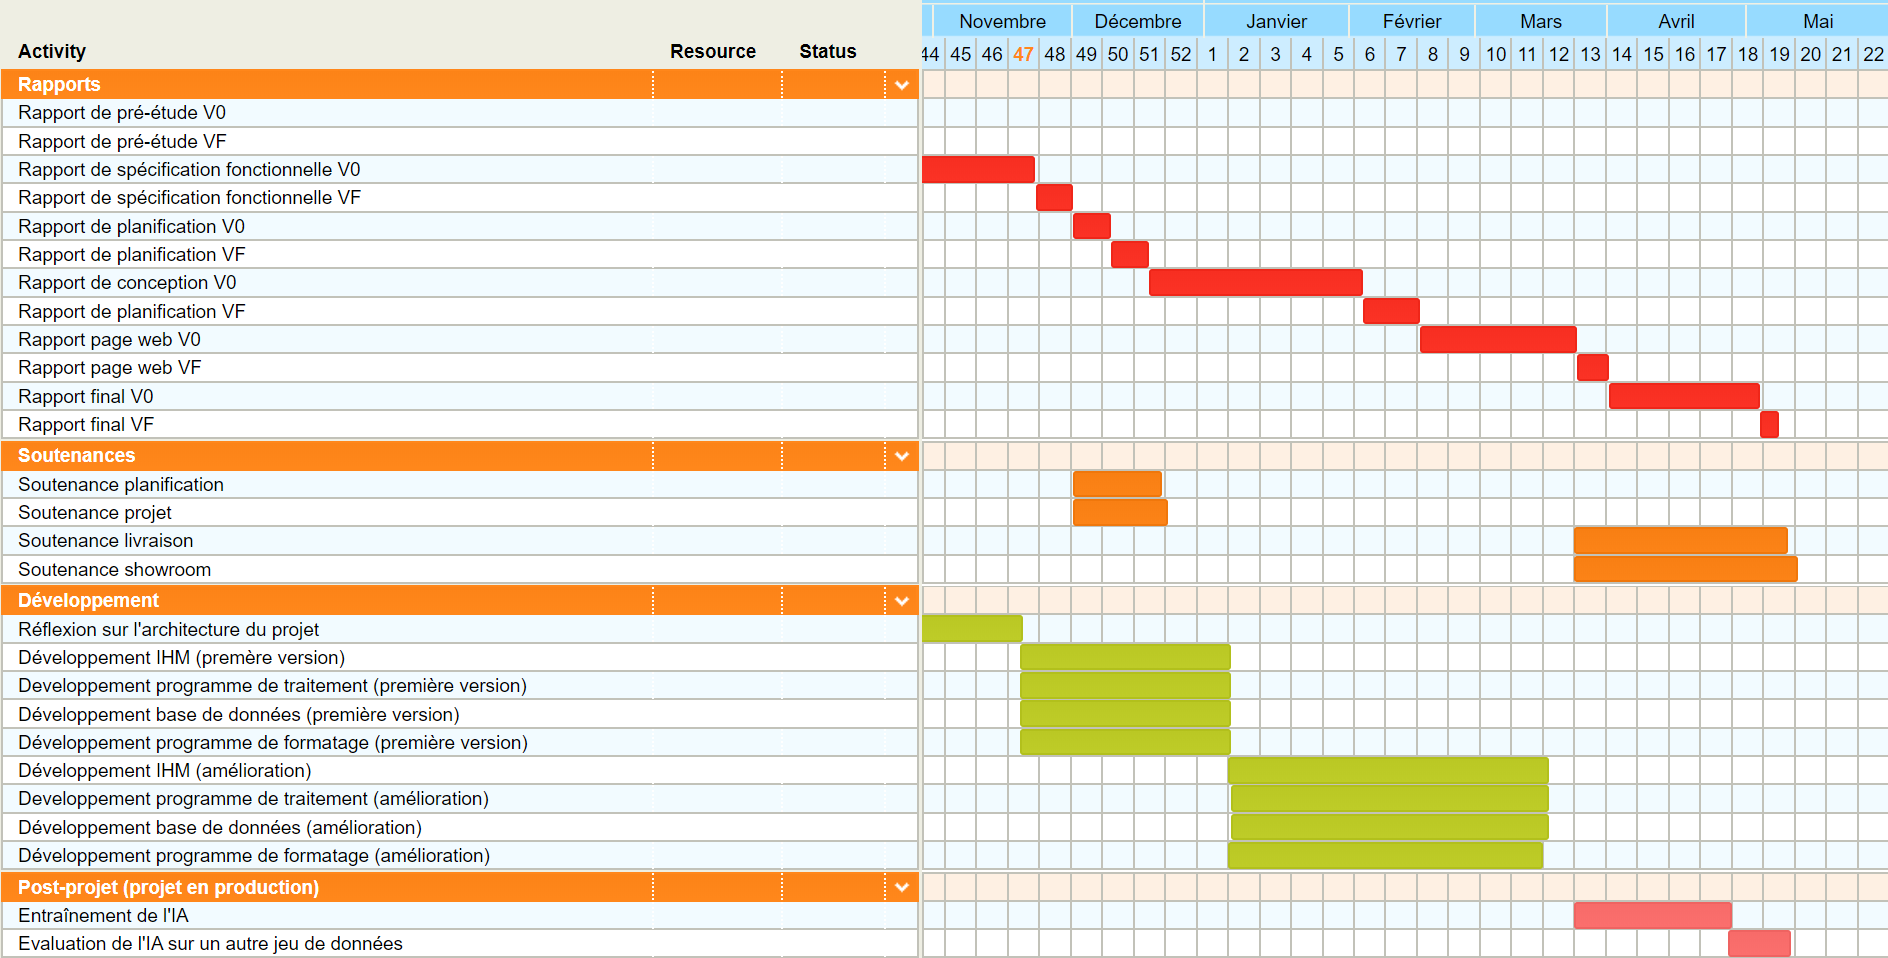
\includegraphics[scale=0.5]{gantt.png}
\end{center}
\end{mdframed}

\paragraph{}
\underline{Légende}

\paragraph{}
\textcolor{red}{En rouge : } rédaction des différents livrables. Nous avons estimé que le début de rédaction d’un livrable doit se faire dès le rendu du livrable précédent.

\paragraph{}
\textcolor{orange}{En orange : } soutenances. Les dates de début de préparation sont pour l’instant difficiles à définir, la taille des blocs est donc provisoire.

\paragraph{}
\textcolor{green}{En vert : } développement. Comme on peut le voir, il y a plusieures parties du développement qui se font en parallèle. Les durées de chaques parties sont prévisionnelles mais sont susceptibles d’être grandement modifiées.

\paragraph{}
\textcolor{pink}{En rose : } exécution du projet en mode production. Ce seront les tests du reconnaisseur.


% ---

\chapter{Conclusion}

Dans le cadre de notre 4\up{ème} année en informatique, nous avons pour mission de
mener à bien un projet de manière plus précise et plus structurée qu’en 3\up{ème} année.
Notre projet, en partenariat avec les archives départementales d’Ille-et-Vilaine,
l’équipe IntuiDoc et Doptim, consiste à créer un logiciel qui aidera les chercheurs et
les ingénieurs à faire progresser la reconnaissance d’écriture manuscrite, afin de rendre
des documents anciens plus accessibles et plus compréhensibles.

\paragraph{}
Notre groupe se compose de 8 étudiants : Enzo CRANCE, Kevin DESPOULAINS, Timothée NEITTHOFFER,
Laure DU MESNILDOT, Charlotte RICHARD, Valentin FOUCHER, Gaël GENDRON et Corentin GUILLOUX.
3 d’entre nous partiront en mobilité internationale au second semestre : Kevin DESPOULAINS,
Gaël GENDRON et Corentin GUILLOUX. Il nous faudra ainsi prendre en compte dans la réalisation
de notre projet ce changement d’effectif. L’étude du projet, la répartition des tâches et la
planification ont donc été faites bien en amont des phases de développement pour permettre à
ceux qui seront encore présents au second semestre de ne pas prendre de retard.

\paragraph{}
Nous avons dans un premier temps étudié ce qui nous était demandé de faire avant de
décider des technologies que nous allions utiliser. Nous avons bien sûr commencé à
étudier les différents outils (langages, API, etc.) que nous pourrions utiliser et qui
feront l’objet du prochain rapport.

\paragraph{}
Nous avons ensuite rédigé notre cahier des charges en reprenant les différentes fonctionnalités
que nous souhaitons développer, en accord avec Bertrand COÜASNON, tout en prenant en compte
les éléments extérieurs avec lesquels notre programme doit communiquer.

\paragraph{}
Nous avons également distribué les rôles qui nous semblent importants pour veiller au bon
déroulement du projet sans mettre trop de pression sur les personnes les endossant.
Un planning prévisionnel a également été rédigé.

%\newpage
%\bibliography{main}
%\bibliographystyle{plain}

%\chapter{Annexes}


\includepdf[pages=-]{pagen.pdf}
\end{document}